% Papel milimetrado A4 — Eric Lucero González — https://ericlucero.dev
% Licencia CC BY-NC-SA 4.0. Compilar con pdfLaTeX.
\documentclass[a4paper]{article}
\usepackage[margin=1cm]{geometry}
\usepackage{tikz}
\usepackage{siunitx}
\pagestyle{empty}

% ── Configuración ──────────────────────────────────────────
\def\widthSqrt{18}      % ancho de la rejilla (cm)
\def\heightSqrt{25}     % alto de la rejilla (cm)
\def\smallSubDiv{0.5}
\def\bigSubDiv{1.0}
\def\biggerSubDiv{5.0}

\begin{document}
\begin{center}
  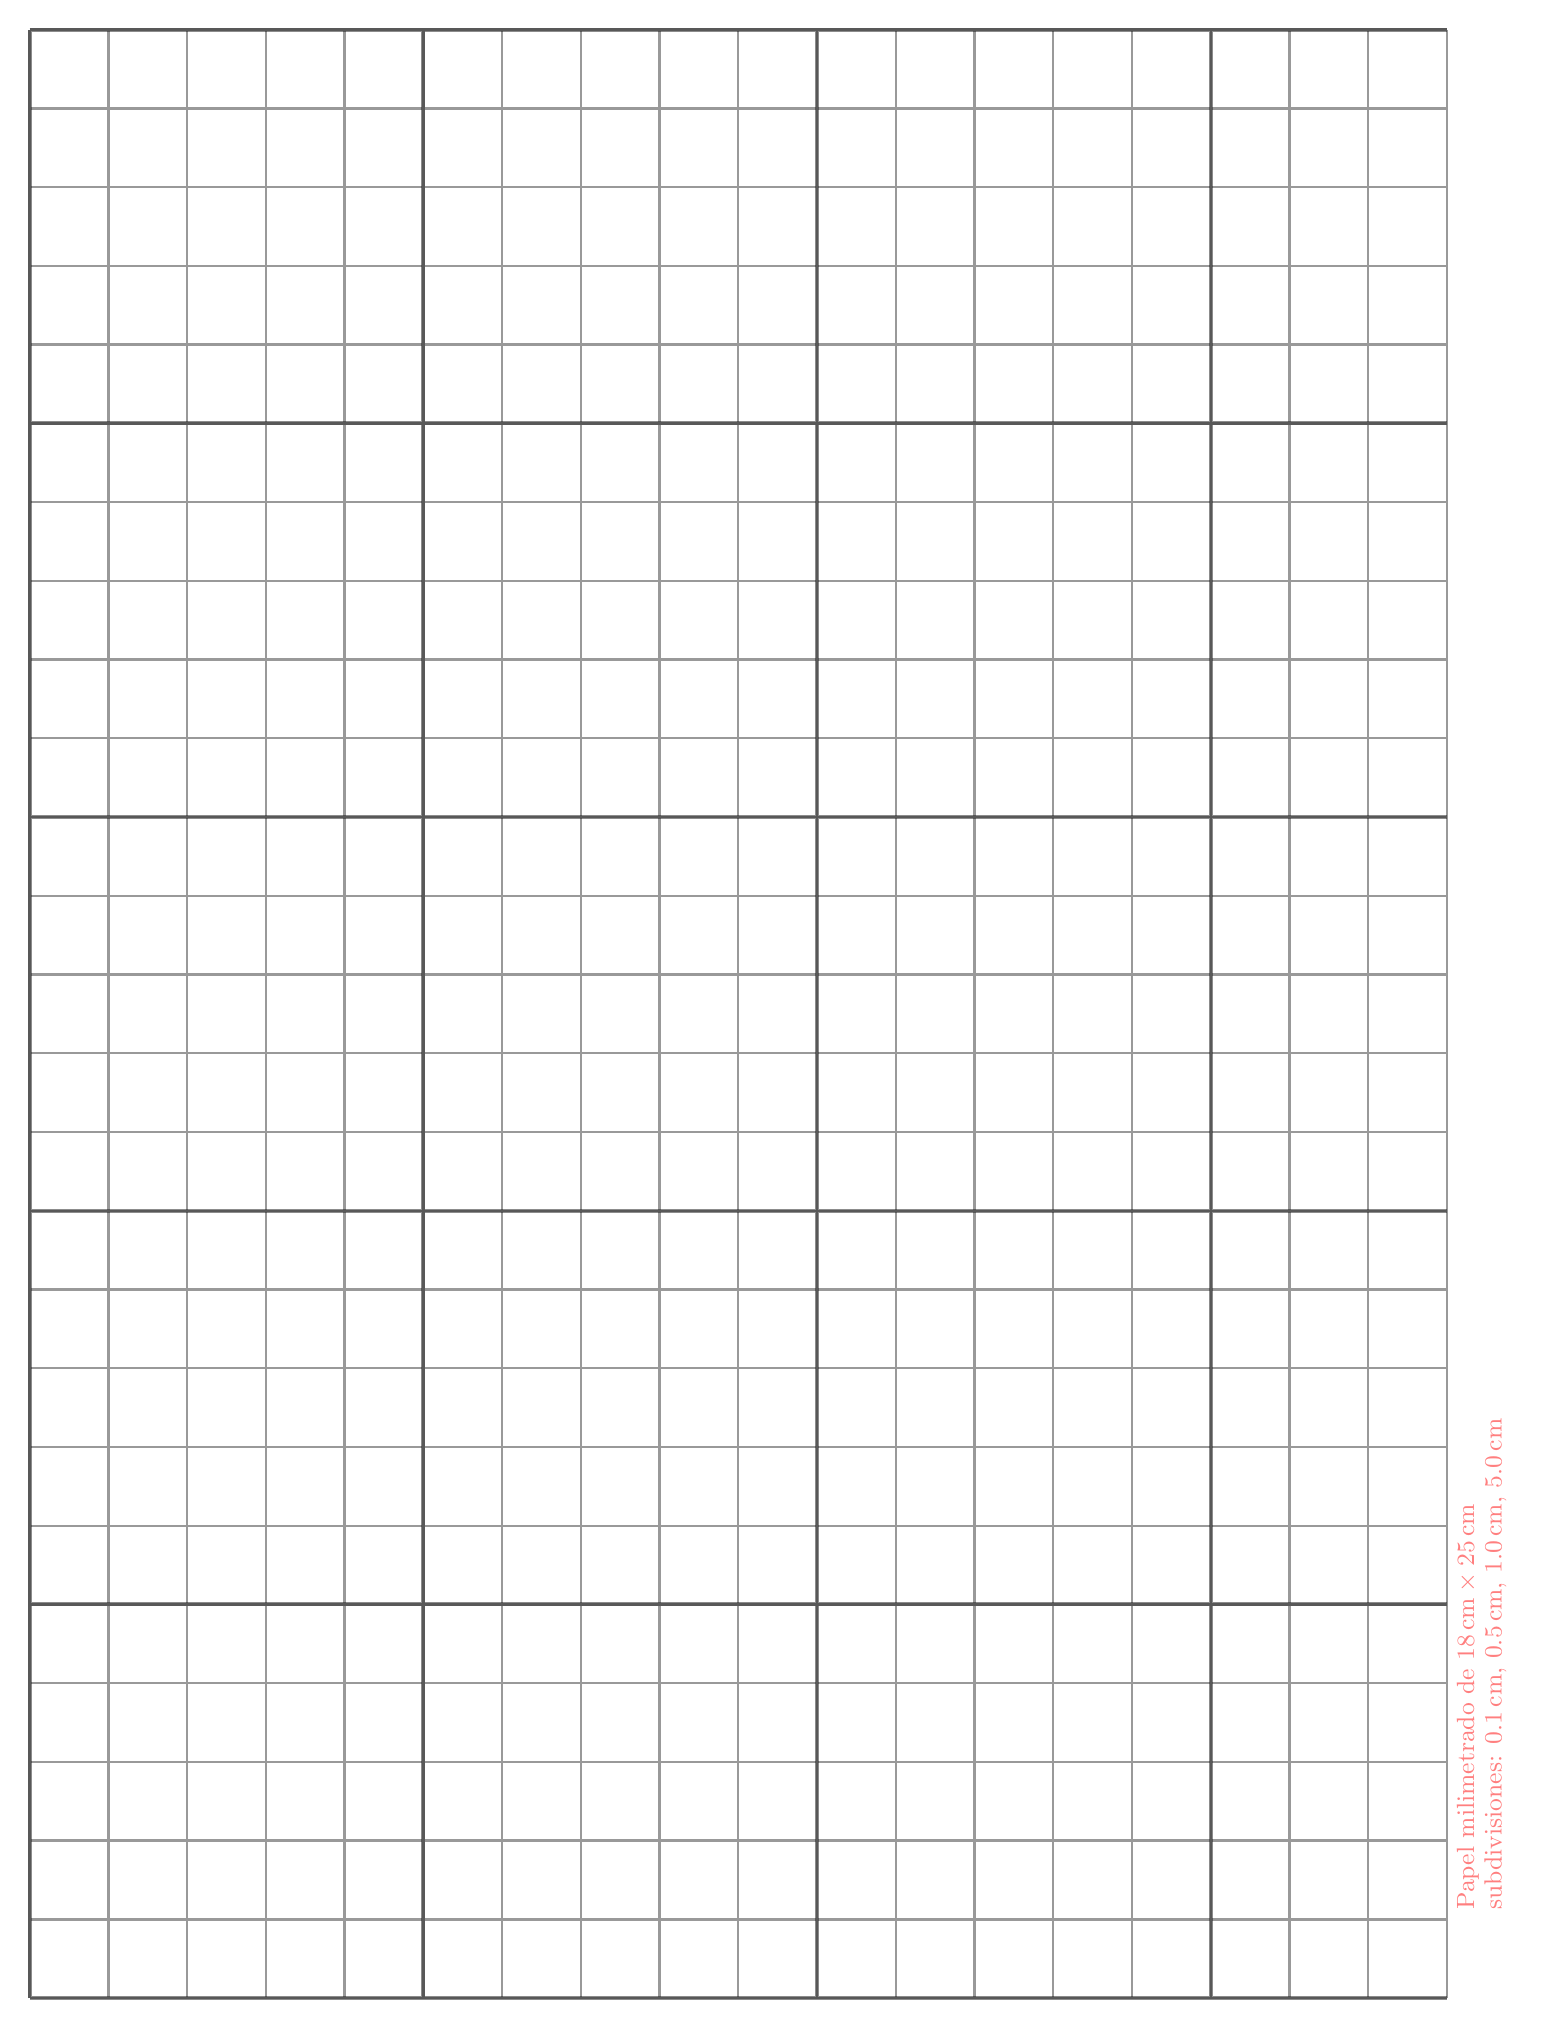
\begin{tikzpicture}[x=1cm, y=1cm, semitransparent]
    % \draw[step=1mm, line width=0.1mm, black!20!white] (0,0) grid (\widthSqrt,\heightSqrt);
    % \draw[step=5mm, line width=0.2mm, black!50!white] (0,0) grid (\widthSqrt,\heightSqrt);
    \draw[step=1cm, line width=0.3mm, black!80!white] (0,0) grid (\widthSqrt,\heightSqrt);
    \draw[step=5cm, line width=0.5mm, black!90!white] (0,0) grid (\widthSqrt,\heightSqrt);
    \node[below right, color=red, rotate=90] at (\widthSqrt,1)
    {\small Papel milimetrado de $\SI{\widthSqrt}{cm} \times \SI{\heightSqrt}{cm}$};
    \node[below right, color=red, rotate=90] at (\widthSqrt+0.35,1)
    {\small subdivisiones: $\SI{0.1}{cm}$, $\SI{\smallSubDiv}{cm}$, $\SI{\bigSubDiv}{cm}$, $\SI{\biggerSubDiv}{cm}$};
  \end{tikzpicture}
\end{center}

\end{document}
